	\chapter{Association schemes}\label{association}
	Association schemes arise in group theory, graph theory, design theory, coding theory and more. For example, if $X$ is a finite group with conjugacy classes $\cC[g] = \{hgh^{-1}:h\in X\}$ ($g\in X$), then the conjugacy class relations $R_g = \left\{ (a,b) \mid ab^{-1} \in \cC[g]  \right\}$ yield a 
	commutative association scheme on the vertex set $X$. The orbits on $X\times X$ of any 
	permutation group $G$ acting generously transitively on a set $X$  give a symmetric association scheme.
	Some of the most well-studied association schemes are distance-regular graphs, including Moore graphs, distance-transitive graphs, strongly regular graphs, generalized polygons, etc. One studies 
	$q$-ary error-correcting codes of length  $n$ as vertex subsets of the Hamming association scheme
	$H(n,q)$ \cite[Sec.~9.2]{Brouwer1989} and one studies $t$-($v,k,\lambda$) designs as vertex subsets of the 
	Johnson association scheme  $J(v,k)$ \cite[Sec.~9.1]{Brouwer1989}.  For an introduction to the 
	extensive literature on the subject, the reader may consult \cite{Delsarte1973,Bannai1984,Brouwer1989,Godsil1993}, 
	the survey \cite{Martin2009}, or the more recent book of  Bailey \cite{Bailey2005} which focuses on 
	connections to the statistical design of experiments.
	
	Let $X$ be a finite set of vertices. A \textit{symmetric d-class association scheme} (see \cite{Brouwer1989}) on $X$ is a pair $\mathcal{L} = (X,\mathcal{R})$ where $\mathcal{R} =\left\{R_0,R_1,\dots,R_d\right\}$ is a set of $d+1$ relations on $X$ satisfying the following properties:
	\begin{enumerate}[label=(\roman*)]
		\item $R_0$ is the identity relation;
		\item $\left\{R_0,R_1,\dots, R_d\right\}$ forms a partition of $X\times X$;
		\item $(x,y)\in R_i$ implies $(y,x)\in R_i$;
		\item for $0\leq i,j,k\leq d$ there exist constants $p_{i,j}^k$ such that for any $(x,y)\in R_k$, the number of vertices $z$ for which $(x,z)\in R_i$ and $(z,y)\in R_j$ is equal to $p_{i,j}^k$ independent of our original choice of $x$ and $y$.
	\end{enumerate}
	The constants $p_{i,j}^k$ are known as the \emph{intersection numbers} of our association scheme and we allow ourselves to suppress the comma whenever $i$ and $j$ are given by single digits, thus $p_{0,7}^6$ and $p_{07}^6$ synonymous but we will never write $p_{102}^2$, instead using $p_{10,2}^2$. Property $(iii)$ and $(iv)$ together imply that $p_{ij}^k = p_{ji}^k$ for all $i,j,k$, thus any symmetric association schemes will be \textit{commutative}. There is a broader definition for an association scheme where we replace $(iii)$ with the requirement that for every $i$, there exists some $j$ such that $R_j = R_i^T$; that is $(x,y)\in R_i$ if and only if $(y,x)\in R_j$. In this case however, we add the additional requirement $p_{ij}^k = p_{ji}^k$ so that our scheme remains commutative. Throughout this text, all association schemes will be symmetric and therefore commutative, but we will add remarks at times when the theorems may be extended to the non-symmetric case.
	
	For each $0\leq i\leq d$ we define the (undirected) graph $\Gamma_i = \Gamma(X,R_i)$ on $X$ with $\Gamma_1,\dots,\Gamma_d$ all simple. For each $a\in X$ we define the $i^\text{th}$ \emph{neighborhood} of $a$ $R_i(a) = \left\{b\in X\vert (a,b)\in R_i\right\}$; i.e. $R_i(a)$ is the neighborhood of $a$ in the graph $\Gamma_i$. Then for any $a\in X$, the set $X$ is partitioned into the \emph{subconstituents} $R_i(a)$ for $0\leq i\leq d$. Consider the following example on $8$ vertices:
	\begin{example} Consider the association scheme called the \emph{3-cube} on vertex set $X = \left\{1,\dots,8\right\}$ with relations corresponding to the graphs $\Gamma_0,\dots,\Gamma_3$ given below.
		\begin{figure}[H]\begin{center}\scalebox{.7}{$\begin{aligned}
		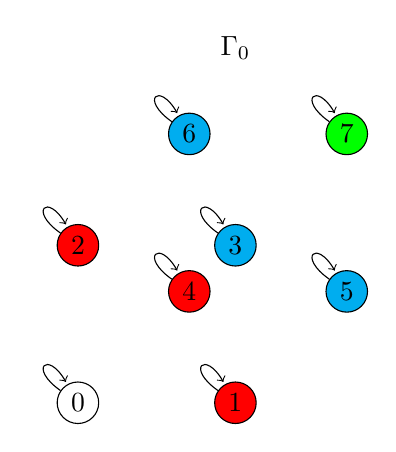
\begin{tikzpicture}[shorten >=1pt,auto,node distance=2cm,
		thin,main node/.style = {circle,draw, inner sep = 0pt, minimum size = 15pt}]
		
		\node[main node,fill=white] (1) {0};
		\node[main node,fill=red] [right of = 1](2) {1};
		\node[main node,fill=red] [above of = 1](3) {2};
		\node[main node,fill=cyan] [right of = 3](4) {3};
		\node[main node,fill=red] [above right of = 1](5) {4};
		\node[main node,fill=cyan] [right of = 5](6) {5};
		\node[main node,fill=cyan] [above of = 5] (7) {6};
		\node[main node,fill=green] [right of = 7](8) {7};
		\node at (2,4.5) (9) {$\Gamma_0$};
		
		\path (1) edge [in=120,out=145,loop] ();
		\path (2) edge [in=120,out=145,loop] ();
		\path (3) edge [in=120,out=145,loop] ();
		\path (4) edge [in=120,out=145,loop] ();
		\path (5) edge [in=120,out=145,loop] ();
		\path (6) edge [in=120,out=145,loop] ();
		\path (7) edge [in=120,out=145,loop] ();
		\path (8) edge [in=120,out=145,loop] ();
		
		\end{tikzpicture}\qquad&\qquad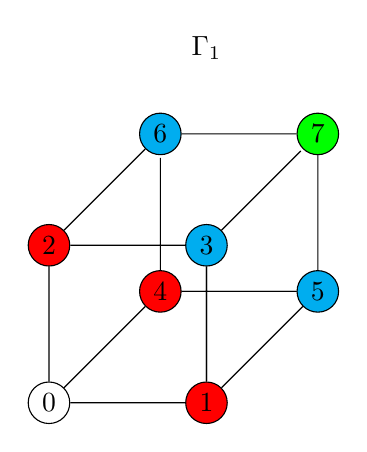
\begin{tikzpicture}[shorten >=1pt,auto,node distance=2cm,
		thin,main node/.style = {circle,draw, inner sep = 0pt, minimum size = 15pt}]
		
		\node[main node,fill=white] (1) {0};
		\node[main node,fill=red] [right of = 1](2) {1};
		\node[main node,fill=red] [above of = 1](3) {2};
		\node[main node,fill=cyan] [right of = 3](4) {3};
		\node[main node,fill=red] [above right of = 1](5) {4};
		\node[main node,fill=cyan] [right of = 5](6) {5};
		\node[main node,fill=cyan] [above of = 5] (7) {6};
		\node[main node,fill=green] [right of = 7](8) {7};
		\node at (2,4.5) (9) {$\Gamma_1$};
		
		\draw[-] (3)--(1)--(2)--(4)--(3)--(7)--(8)--(6)--(5)--(7);
		\draw[-] (1)--(5)--(6)--(2)--(4)--(8);
		\end{tikzpicture}\qquad\qquad
		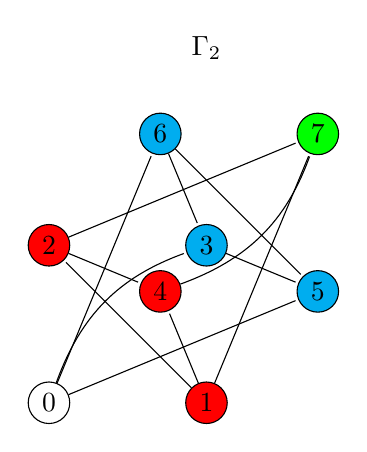
\begin{tikzpicture}[shorten >=1pt,auto,node distance=2cm,
		thin,main node/.style = {circle,draw, inner sep = 0pt, minimum size = 15pt}]
		
		\node[main node,fill=white] (1) {0};
		\node[main node,fill=red] [right of = 1](2) {1};
		\node[main node,fill=red] [above of = 1](3) {2};
		\node[main node,fill=cyan] [right of = 3](4) {3};
		\node[main node,fill=red] [above right of = 1](5) {4};
		\node[main node,fill=cyan] [right of = 5](6) {5};
		\node[main node,fill=cyan] [above of = 5] (7) {6};
		\node[main node,fill=green] [right of = 7](8) {7};
		\node at (2,4.5) (9) {$\Gamma_2$};
		
		\path[-]
		(1)edge [bend left=25] node {} (4)
		edge node {} (6)
		edge node {} (7)
		(2)edge node {} (3)
		edge node {} (5)
		edge node {} (8)
		(3)edge node {} (5)
		edge node {} (8)
		(4) edge node {} (6)
		(7) edge node {} (4)
		edge node {} (6)
		(5) edge [bend right = 25] node {} (8);
		\end{tikzpicture}\qquad&\qquad
		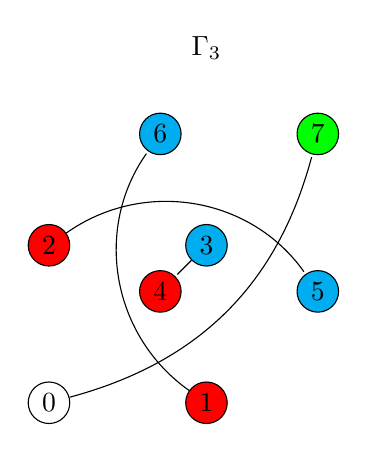
\begin{tikzpicture}[shorten >=1pt,auto,node distance=2cm,
		thin,main node/.style = {circle,draw, inner sep = 0pt, minimum size = 15pt}]
		
		\node[main node,fill=white] (1) {0};
		\node[main node,fill=red] [right of = 1](2) {1};
		\node[main node,fill=red] [above of = 1](3) {2};
		\node[main node,fill=cyan] [right of = 3](4) {3};
		\node[main node,fill=red] [above right of = 1](5) {4};
		\node[main node,fill=cyan] [right of = 5](6) {5};
		\node[main node,fill=cyan] [above of = 5] (7) {6};
		\node[main node,fill=green] [right of = 7](8) {7};
		\node at (2,4.5) (9) {$\Gamma_3$};
		
		\path[-]
		(1) edge [bend right] node {} (8)
		(2) edge [bend left=45] node {} (7)
		(3) edge [bend left=45] node {} (6)
		(4) edge node {} (5);
		\end{tikzpicture}
		\end{aligned}$}\end{center}
		\caption[Graphs of the 3-cube.]{The four graphs of the 3-cube. The four subconstituents of the vertex $0$ are colored white, red, blue, and green respectively.}\label{3cube}
		\end{figure}
		The intersection numbers of this association scheme are as follows where the $i^\text{th}$ matrix list $p^k_{ij}$ with rows indexed by $k$ and columns indexed by $j$:
		\[\left[\begin{array}{cccc}
		1&0&0&0\\
		0&1&0&0\\
		0&0&1&0\\
		0&0&0&1\\
		\end{array}\right],\left[\begin{array}{cccc}
		0&3&0&0\\
		1&0&2&0\\
		0&2&0&1\\
		0&0&3&0\\
		\end{array}\right],\left[\begin{array}{cccc}
		0&0&3&0\\
		0&2&0&1\\
		1&0&2&0\\
		0&3&0&0\\
		\end{array}\right],\left[\begin{array}{cccc}
		0&0&0&1\\
		0&0&1&0\\
		0&1&0&0\\
		1&0&0&0\\
		\end{array}\right].\]
		Since $p^k_{ij} = p^k_{ji}$ we note that many of the columns listed above are repeated, thus we may instead give a more brief list of the intersection numbers as follows:
		\[\begin{array}{c|cccc|ccc|cc|c}
		j & p^{j}_{0,0}	&p^{j}_{0,1}& p^{j}_{0,2} 	& p^{j}_{0,3}   & p^{j}_{1,1}	&p^{j}_{1,2}& p^{j}_{1,3} 	& p^{j}_{2,2} 	& p^{j}_{2,3} 	& p^{j}_{3,3}\\\hline
		0 & 1			& 0			& 0 			& 0				& 3				& 0			& 0 			& 3				& 0   			& 1\\
		1 & 0			& 1			& 0 			& 0				& 0				& 2			& 0 			& 0   			& 1   			& 0\\
		2 & 0			& 0			& 1 			& 0				& 2				& 0 		& 1				& 2 			& 0 			& 0\\
		3 & 0			& 0			& 0 			& 1				& 0 			& 3			& 0 			& 0   			& 0 			& 0\\
		\end{array}\]
		We will often find this brief description useful and will further reduce our description of the parameters in many of the examples we give where possible.
	\end{example}
	For any $0\leq i\leq d$ and any vertex $x\in X$,
	\[p^{0}_{ii} = \left\vert\left\{y:(y,x)\in R_i\right\}\right\vert = \left\vert R_i(x)\right\vert.\]
	Thus we define $k_i:=p^0_{ii}$ as the \emph{valency} of the $i^\text{th}$ relation. Many other restrictions on our intersection numbers follows immediately from our definition, for instance $p^0_{12} = 0$; we will summarize these in a latter lemma.
	\section{Bose-Mesner algebra}
	Often it becomes useful to order the vertices in $X$ and then represent each $R_i$ as a 01-matrix $A_i$ where the $(x,y)$ entry of $A_i$ is 1 if and only if $(x,y)\in R_i$, thus $A_i$ is the adjacency matrix of $\Gamma_i$. The defining properties of an association scheme are then encoded as:
	\begin{enumerate}[label=(\roman*)]
		\item $A_0 = I$;
		\item $\sum_i A_i = J$;
		\item for all $0\leq i\leq d$, $A_i^T = A_i$;
		\item for all $0\leq i,j\leq d$, $A_iA_j = \sum p_{i,j}^k A_k$.
	\end{enumerate}
	The fourth condition tells us that $\BMA = \text{span}\left\{A_0,A_1,\dots A_d\right\}$ forms a matrix algebra under standard matrix multiplication. We call this algebra the \emph{Bose-Mesner algebra} and note that the remaining conditions ensure it is a $(d+1)$-dimensional algebra of symmetric matrices containing the identity. Further, as our basis matrices are 01-matrices with disjoint support, this algebra is also closed under Schur (element-wise) products. Since $p^k_{ij} = p^k_{ji}$ for all $i,j,k$, we must have $A_iA_j = A_jA_i$, that is our algebra is also commutative. Therefore we may simultaneously diagonalize the matrices $\left\{A_0,\dots,A_d\right\}$ using the maximal common orthogonal eigenspaces $V_0,\dots,V_{d'}$ with corresponding idempotents $E_0,\dots,E_{d'}$. Since, for every $i$, there exists eigenvalues $\theta_{ij}$ such that $A_i = \sum_{j=0}^{d'}\theta_{ij}E_j$ we find that $\BMA \subseteq \text{span}\left\{E_0,E_1,\dots, E_{d'}\right\}$ thus $d\leq d'$. Further since the eigenspaces $V_j$ are maximal for each $0\leq j\leq d$ and pairwise orthogonal,
	\[E_j = \frac{1}{c_j}\prod_{i=0}^d\left(\prod_{\theta_{ik}\neq\theta_{ij}}\left(A_i-\theta_{ik}I\right)\right)\]
	for some normalization constant $c_j$. Thus $E_j\in \BMA$ giving $\text{span}\left\{E_0,E_1,\dots, E_{d'}\right\}\subseteq\BMA$ and therefore $d=d'$. Then, for any $d$-class association scheme there is a basis of exactly $d+1$ idempotents $E_0,\dots,E_d$ which are unique up to reordering and diagonalize every matrix in $\BMA$. Since $J\in\BMA$, the rank 1 idempotent $\frac{1}{\vert X\vert}J$ must be contained within this basis; by convention we assume $E_0= \frac{1}{\vert X\vert}J$. We take a moment here to remark on the notion of duality in our matrix algebra. We have already mentioned that $\BMA$ is closed under two distinct products: standard matrix multiplication and Schur multiplication. While it is clear these are distinct products, consider an abstract vector space with basis vectors $\left\{b_i\right\}$. For any pair of vectors $v = \sum_i v_ib_i$ and $w = \sum_i w_ib_i$, we may define the \emph{product with respect to basis $\left\{b_i\right\}$} as $v\star w = \sum_i (v_iw_i)b_i$. In this light, our two distinct products become very similar; for $F,F'\in\BMA$ with $F = \sum_if_iE_i = \sum_i g_iA_i$ and $F' = \sum_if_i'E_i = \sum_i g_i'A_i$, we have
	\[\begin{aligned}
	FF' & =\sum_i\sum_jf_if_j'E_iE_j = \sum_i f_if_i'E_i,\\
	F\circ F' &=\sum_i\sum_jg_ig_i'A_i\circ A_j= \sum_i g_ig_i'A_i.
	\end{aligned}\]
	Therefore our distinct products may be described as the product with respect to the basis $\left\{E_i\right\}$ (standard matrix multiplication) and the product with respect to the basis $\left\{A_i\right\}$ (elementise multiplication). Thus we consider our two products similar and will often refer to them as dual operations on our algebra. Further, we consider the basis matrices $A_0,\dots,A_d$ and $E_0,\dots,E_d$ ``dual" in a sense. Throughout this work, we will often be interested in investigating this duality and pointing out when there are differences and/or gaps in our understanding of the landscape. Our first consideration regarding these two bases for our algebra is the change of basis matrices between the two. Since both $\left\{A_0,\dots,A_d\right\}$ and $\left\{E_0,\dots,E_d\right\}$ form bases $\BMA$, there exists unique matrices $P$ and $Q$ so that
	\begin{equation}
	\label{PQmat}
	A_i = \sum_{j} P_{ji} E_j,\qquad E_j = \frac{1}{\vert X\vert} \sum_{i} Q_{ij}A_i.
	\end{equation}
	We call $P$ and $Q$ the first and second eigenmatrices, noting that the eigenvalues of $A_i$ are given by column $i$ of $P$ and the ``dual eigenvalues" of $\vert X\vert E_j$, that is eigenvalues with respect to the Schur product, are given by column $j$ of $Q$. Let $\Delta_m=\text{diag}(m_0,m_1,\dots,m_d)$ and $\Delta_k=\text{diag}(k_0,k_1,\dots,k_d)$ and the following two relations hold for our eigenmatrices:
	\begin{lem}[\cite{Brouwer1989}, First and second orthogonality relations] The matrices $P$ and $Q$ of an association scheme satisfy:
		\begin{equation}
		PQ = \vert X\vert I, \qquad \Delta_mP = Q^T\Delta_k
		\end{equation}
	\end{lem}
	A second consideration for our dual bases is that while we used the existence of structure constants $p^k_{ij}$ to show that $\BMA$ was closed under matrix multiplication, closure under Schur products came from the fact that each $A_i$ was idempotent under this product. This additional closure implies the existence of structure constants for our second basis. That is, for $0\leq i,j,k\leq d$ there exists constants $q^k_{ij}$ so that
	\begin{equation}E_i\circ E_j = \frac{1}{\vert X\vert}\sum_k q_{i,j}^k E_k.\label{Emult}\end{equation}
	We call these constants the \emph{Krein paramters} of the association scheme. Here we list many of the properties of both the intersection numbers and the Krein parameters, including our first and second eigenmatrices as well. See lemmas 2.1.1, 2.2.1, and 2.3.1 for proofs of the following lemma.
	\begin{lem}[{\cite{Brouwer1989}}]\label{kitchensink} The parameters $p^\ell_{ij}$, $q^\ell_{ij}$, $k_i = p^0_{ii}$, $m_j = q^0_{jj}$, and the eigenmatrices $P$ and $Q$ satisfy:
		\begin{multicols}{2}
		\begin{enumerate}
			\item[(i)] $p_{0j}^\ell = \delta_{j\ell}$,
			\item[(ii)] $p^0_{ij} = \delta_{ij}k_i$,
			\item[(iii)] $p^\ell_{ij} = p^\ell_{ji}$,
			\item[(iv)] $p^\ell_{ij}k_\ell= p^j_{i\ell}k_j$,
			\item[(v)] $\sum_jp^\ell_{ij} = k_j$,
			\item[(vi)] $\sum_\ell p^\ell_{ij}p^m_{\ell h} = \sum_\ell p^m_{i\ell}p^\ell_{jh}$.
			\item[(vii)] $P_{ij}P_{ih} = \sum_\ell p^\ell_{jh}P_{i\ell}$,
			\item[(viii)] $P_{ji}Q_{hj} = \sum_\ell p_{i\ell}^hQ_{\ell j}$,
			\item[(ix)] $\sum_{j}P_{ji} = \sum_{h}p^h_{hi}$,
			\item[(x)] $P_{j0} = 1$,
			\item[(xi)] $P_{0i} = k_i$,
			\item[(xii)] $\sum_j m_jP_{ji}P_{jh} = \vert X\vert k_i\delta_{ih}$,
				
			\item[($i^\prime$)] $q^\ell_{0j} = \delta_{j\ell}$,
			\item[($ii^\prime$)] $q^0_{ij} = \delta_{ij}m_j$,
			\item[($iii^\prime$)] $q^{\ell}_{ij} = q^\ell_{ji}$,
			\item[($iv^\prime$)] $q^\ell_{ij}m_\ell = q^j_{i\ell}m_j$,
			\item[($v^\prime$)] $\sum_j q^\ell_{ij} = m_i$,
			\item[($vi^\prime$)] $\sum_\ell q^\ell_{ij}q^{m}_{\ell k} = \sum_\ell q^m_{i\ell}q^\ell_{jk}$,
			\item[($vii^\prime$)] $Q_{ij}Q_{ih} = \sum_{\ell}q^\ell_{jh}Q_{i\ell}$,
			\item[($viii^\prime$)] $P_{ij}Q_{jh} = \sum_\ell q^i_{h\ell}P_{\ell j}$,
			\item[($ix^\prime$)] $\sum_{j}Q_{ji} = \sum_{h}q^h_{hi}$,
			\item[($x^\prime$)] $Q_{i0} = 1$,
			\item[($xi^\prime$)] $Q_{0j} = m_j$,
			\item[($xii^\prime$)] $\sum_j k_iQ_{ij}Q_{ih} = \vert X\vert m_j\delta_{jh}$,
		\end{enumerate}
		\end{multicols}
	\end{lem}
	\section{Parameter arrays}
	For a matrix $A$, we denote the entry in row $i$ and column $j$ as $\left[A\right]_{ij}$. We define the \emph{arrays of intersection numbers} $L_0,\dots,L_d$ as $(d+1)\times(d+1)$ matrices where $\left[L_i\right]_{k,j} = p^k_{ij}$. We then define the vector space $\bbL = \text{span}\left\{L_0,\dots,L_d\right\}$ and note that Lemma \ref{kitchensink} $(vi)$ gives us that
	\[
	\left[L_iL_j\right]_{m,k} = \sum_lp^m_{il}p^l_{jk} = \sum_{l}p^l_{ij}p^m_{lk} = \sum_l p^l_{ij}\left[L_l\right]_{m,k}
	\]
	for $0\leq m,k\leq d$. Therefore we find that this vector space forms a matrix algebra under matrix multiplication via
	\begin{equation}\label{Lprod}
	L_iL_j = \sum_l p^l_{ij}L_l.
	\end{equation}
	Likewise we define the \emph{arrays of Krein parameters} as $L_0^*,\dots,L_d^*$ with $\left[L_i^*\right]_{k,j} = q^k_{ij}$. This provides a dual matrix algebra $\bbL^* = \text{span}\left\{L_0^*,\dots,L_d^*\right\}$ as Lemma \ref{kitchensink} $(vi^\prime)$ gives
	\begin{equation}\label{Lstarprod}
	L_i^*L_j^* = \sum_{l}q^l_{ij}L_l^*.
	\end{equation}
	In both cases, we may define an algebra isomorphism $\phi:\BMA\rightarrow\bbL$ or $\phi^*:\BMA\rightarrow\bbL^*$ via the basis mappings
	\begin{equation}
		\phi(A_i) = L_i\qquad \phi^*(E_i) = L_i^*.
	\end{equation}
	Note that the first isomorphism preserves standard matrix multiplication while the second preserves Schur products. We will refer to $L_1$ as the \emph{intersection matrix} and $L_1^*$ as the \emph{Krein matrix}. These these two matrices will become especially important for polynomial schemes (see Section \ref{ppoly} and \ref{qpoly}) where they are tridiagonal. We end this section by noting that the matrices given in Example \ref{3cube} were exactly the arrays of intersection numbers for that association scheme. A final note before moving on is that the parameters of an association scheme need not define the scheme uniquely. In fact, there exists non-isomorphic $2$-class association schemes with exactly the same parameters--consider the $4\times 4$ rook graph and Shrikhande graph.
	\section{Example Duality}\label{dualpair}
	In this section, we give an explicit example of the duality mentioned previously. Consider first the strongly regular graph given by $K_{3,3}$. This corresponding association scheme is a 2-class bipartite scheme with nontrivial relations given by adjacency in $K_{3,3}$ and non-adjacency in $K_{3,3}$ respectively. Thus the three graphs for this scheme are as follows:
		\begin{figure}[H]\begin{center}\scalebox{.7}{$\begin{aligned}
				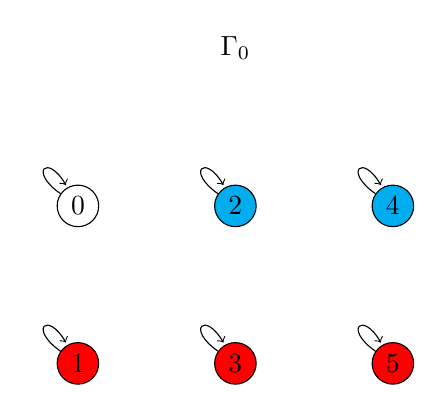
\begin{tikzpicture}[shorten >=1pt,auto,node distance=2cm,
				thin,main node/.style = {circle,draw, inner sep = 0pt, minimum size = 15pt}]
				
				\node[main node,fill=white] (1) {0};
				\node[main node,fill=cyan] [right of = 1](2) {2};
				\node[main node,fill=cyan] [right of = 2](3) {4};
				\node[main node,fill=red] [below of = 1](4) {1};
				\node[main node,fill=red] [right of = 4](5) {3};
				\node[main node,fill=red] [right of = 5](6) {5};
				\node [above of =2] (9) {$\Gamma_0$};
				
				\path (1) edge [in=120,out=145,loop] ();
				\path (2) edge [in=120,out=145,loop] ();
				\path (3) edge [in=120,out=145,loop] ();
				\path (4) edge [in=120,out=145,loop] ();
				\path (5) edge [in=120,out=145,loop] ();
				\path (6) edge [in=120,out=145,loop] ();
				
				\end{tikzpicture}\qquad&\qquad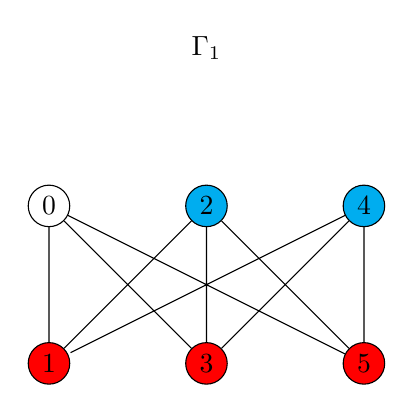
\begin{tikzpicture}[shorten >=1pt,auto,node distance=2cm,
				thin,main node/.style = {circle,draw, inner sep = 0pt, minimum size = 15pt}]
				
				\node[main node,fill=white] (1) {0};
				\node[main node,fill=cyan] [right of = 1](2) {2};
				\node[main node,fill=cyan] [right of = 2](3) {4};
				\node[main node,fill=red] [below of = 1](4) {1};
				\node[main node,fill=red] [right of = 4](5) {3};
				\node[main node,fill=red] [right of = 5](6) {5};
				\node [above of =2] {$\Gamma_1$};
				
				\draw[-] (1)--(4)--(2)--(5)--(3)--(6)--(1)--(5)--(2)--(6)--(3)--(4);
				\end{tikzpicture}\qquad\qquad
				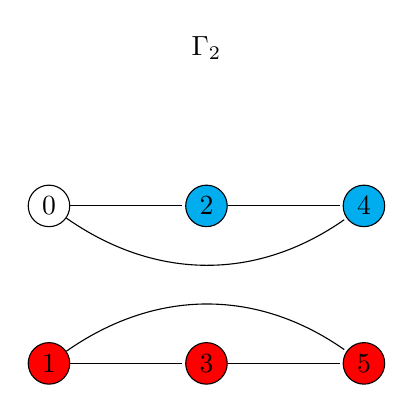
\begin{tikzpicture}[shorten >=1pt,auto,node distance=2cm,
				thin,main node/.style = {circle,draw, inner sep = 0pt, minimum size = 15pt}]	
				\node[main node,fill=white] (1) {0};
				\node[main node,fill=cyan] [right of = 1](2) {2};
				\node[main node,fill=cyan] [right of = 2](3) {4};
				\node[main node,fill=red] [below of = 1](4) {1};
				\node[main node,fill=red] [right of = 4](5) {3};
				\node[main node,fill=red] [right of = 5](6) {5};
				\node [above of =2] {$\Gamma_2$};
				
				\path[-]
				(1)edge node {} (2)
				edge [bend right=35] node {} (3)
				(2)edge node {} (3)
				(4)edge node {} (5)
				edge [bend left=35] node {} (6)
				(5) edge node {} (6);
				\end{tikzpicture}
				\end{aligned}$}\end{center}
		\caption[Graphs of $K_{3,3}$.]{The three graphs of $K_{3,3}$. The subconstituents of vertex $0$ are colored white, red,  and blue respectively.}\label{k33}
	\end{figure}
	The intersection numbers, Krein parameters, and eigenmatrices of this association scheme are as follows:
	\[\begin{aligned}L_0 &= \left[\begin{array}{cccc}
	1&0&0\\
	0&1&0\\
	0&0&1\\
	\end{array}\right],\quad L_1 &= \left[\begin{array}{cccc}
	0&3&0\\
	1&0&2\\
	0&3&0\\
	\end{array}\right],\quad L_2 &= \left[\begin{array}{cccc}
	0&0&2\\
	0&2&0\\
	1&0&1\\
	\end{array}\right];\\
	L_0^* &= \left[\begin{array}{cccc}
	1&0&0\\
	0&1&0\\
	0&0&1\\
	\end{array}\right],\quad L_1^* &= \left[\begin{array}{cccc}
	0&4&0\\
	1&2&1\\
	0&4&0\\
	\end{array}\right],\quad L_2^* &= \left[\begin{array}{cccc}
	0&0&1\\
	0&1&0\\
	1&0&0\\
	\end{array}\right];\end{aligned}\]
	\[P = \left[\begin{array}{cccc}
	1&3&2\\
	1&0&-1\\
	1&-3&2\\
	\end{array}\right],\qquad Q = \left[\begin{array}{cccc}
	1&4&1\\
	1&0&-1\\
	1&-2&1\\
	\end{array}\right].\]
	Now consider the second $2$-class association scheme given by the vertices of the octahedron where the two nontrivial relations are given by sharing an edge in the platonic solid and not sharing an edge respectively. The three graphs for this scheme are as follows:
	\begin{figure}[H]\begin{center}\scalebox{.7}{$\begin{aligned}
				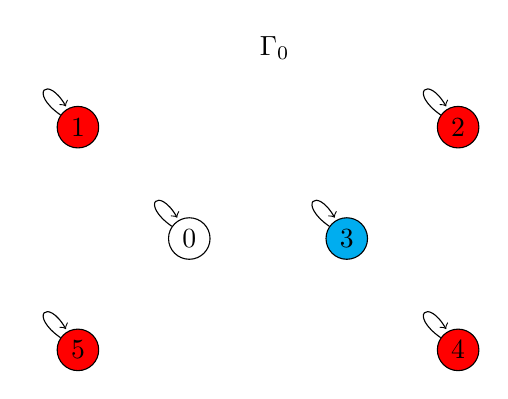
\begin{tikzpicture}[shorten >=1pt,auto,node distance=2cm,
				thin,main node/.style = {circle,draw, inner sep = 0pt, minimum size = 15pt}]
				
				\node[main node,fill=red] (2) {1};
				\node[main node,fill=white] [below right of = 2](1) {0};
				\node[main node,fill=cyan] [right of = 1](6) {3};
				\node[main node,fill=red] [above right of = 6](3) {2};
				\node[main node,fill=red] [below right of = 6](4) {4};
				\node[main node,fill=red] [below left of  = 1](5) {5};
				\node at (2.5,1) (9) {$\Gamma_0$};
				
				\path (1) edge [in=120,out=145,loop] ();
				\path (2) edge [in=120,out=145,loop] ();
				\path (3) edge [in=120,out=145,loop] ();
				\path (4) edge [in=120,out=145,loop] ();
				\path (5) edge [in=120,out=145,loop] ();
				\path (6) edge [in=120,out=145,loop] ();
				
				\end{tikzpicture}\qquad&\qquad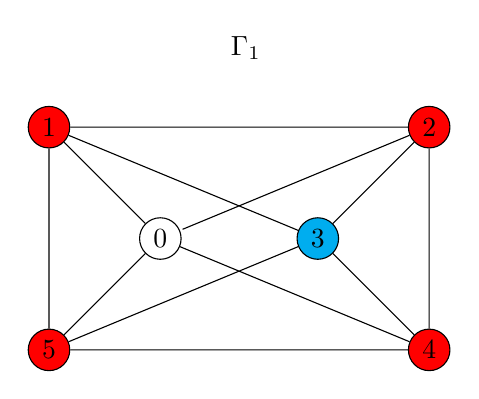
\begin{tikzpicture}[shorten >=1pt,auto,node distance=2cm,
				thin,main node/.style = {circle,draw, inner sep = 0pt, minimum size = 15pt}]
				
				\node[main node,fill=red] (2) {1};
				\node[main node,fill=white] [below right of = 2](1) {0};
				\node[main node,fill=cyan] [right of = 1](6) {3};
				\node[main node,fill=red] [above right of = 6](3) {2};
				\node[main node,fill=red] [below right of = 6](4) {4};
				\node[main node,fill=red] [below left of  = 1](5) {5};
				\node at (2.5,1) (9) {$\Gamma_1$};
				
				\draw[-] (1)--(2)--(3)--(4)--(5)--(2)--(6)--(5)--(1)--(4)--(6)--(3)--(1);
				\end{tikzpicture}\qquad\qquad
				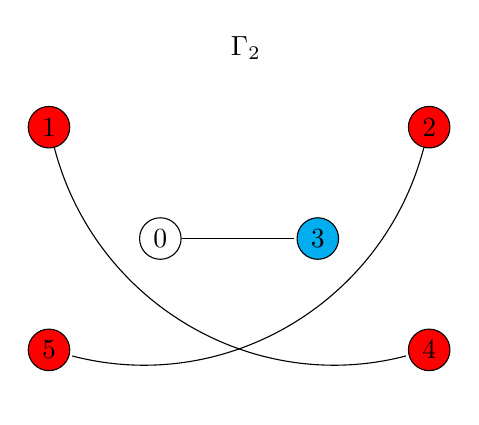
\begin{tikzpicture}[shorten >=1pt,auto,node distance=2cm,
				thin,main node/.style = {circle,draw, inner sep = 0pt, minimum size = 15pt}]	
				
				\node[main node,fill=red] (2) {1};
				\node[main node,fill=white] [below right of = 2](1) {0};
				\node[main node,fill=cyan] [right of = 1](6) {3};
				\node[main node,fill=red] [above right of = 6](3) {2};
				\node[main node,fill=red] [below right of = 6](4) {4};
				\node[main node,fill=red] [below left of  = 1](5) {5};
				\node at (2.5,1) (9) {$\Gamma_2$};
				
				\path[-]
				(1)edge node {} (6)
				(2)edge [bend right=45] node {} (4)
				(3)edge [bend left=45] node {} (5);
				\end{tikzpicture}
				\end{aligned}$}\end{center}
		\caption[Graphs of the octahedron.]{The three graphs of the octahedron. The subconstituents of vertex $0$ are colored white, red, and blue respectively.}\label{octahedron}
	\end{figure}
	The intersection numbers, Krein parameters, and eigenmatrices of this association scheme are as follows:
	\[\begin{aligned}
	L_0 &= \left[\begin{array}{cccc}
	1&0&0\\
	0&1&0\\
	0&0&1\\
	\end{array}\right],\quad L_1 &= \left[\begin{array}{cccc}
	0&4&0\\
	1&2&1\\
	0&4&0\\
	\end{array}\right],\quad L_2 &= \left[\begin{array}{cccc}
	0&0&1\\
	0&1&0\\
	1&0&0\\
	\end{array}\right];\\
	L_0^* &= \left[\begin{array}{cccc}
	1&0&0\\
	0&1&0\\
	0&0&1\\
	\end{array}\right],\quad L_1^* &= \left[\begin{array}{cccc}
	0&3&0\\
	1&0&2\\
	0&3&0\\
	\end{array}\right],\quad L_2^* &= \left[\begin{array}{cccc}
	0&0&2\\
	0&2&0\\
	1&0&1\\
	\end{array}\right];
	\end{aligned}\]
	\[P = \left[\begin{array}{cccc}
	1&4&1\\
	1&0&-1\\
	1&-2&1\\
	\end{array}\right],\qquad Q = \left[\begin{array}{cccc}
	1&3&2\\
	1&0&-1\\
	1&-3&2\\
	\end{array}\right].\]
	One may observe that the intersection numbers and the Krein parameters of the two schemes are interchanged as well as the first and second eigenmatrices. This is, in part, due to a duality arising from the context of translation schemes: schemes for which there exists an abelian group $G$ acting transitively on the vertices with $(g(x),g(y))\in R_i$ if and only if $(x,y)\in R_i$ for every $x,y\in X$ and $g\in G$. When this occurs we may define a dual association scheme (which is also a translation scheme) $(\hat{X},\hat{\mathcal{R}})$ where $\hat{X} = \left\{\chi:\chi\in G^*\right\}$ and $(\chi,\chi')\in \hat{R}_i$ if and only if $E_i (\chi-\chi') = (\chi-\chi')$. In the case of the two association schemes given above, $G\simeq Z_6$ and building the dual scheme of one will result in the other.
	
	In general we often find the automorphism group of an association scheme to be trivial, and thus certainly do not expect to find a transitive action on the vertices. However the duality still persists at times in the formal sense. Therefore we say two association schemes are \emph{formally dual} if swaping the eigenmatrices of one gives the eigenmatrices of the other (equivalently swapping the intersection numbers and Krein parameters of one gives the parameters of the other). We often find that no dual scheme may exist (consider any association scheme for which the Krein parameters are not integral), however this notion of formal duality still plays a major role in our understanding of the field of association schemes as a whole. It will motivative many of the questions which we will focus on in this thesis. We finish this example with one final note: any parameter level definition will often bring rise to similar definitions for the dual. For instance we find that $K_{3,3}$ is bipartite because $p^k_{ij}= 0$ whenever $i+j+k\notin2\bbZ$. Then the dual graph, the octahedron, follows $q^k_{ij}=0$ whenever $i+j+k\notin2\bbZ$ and we will call this ``dual-bipartite" or $Q$-bipartite (see \ref{qbip}). Similarly we find that both $K_{3,3}$ and the octahedron are ``antipodal graphs": $p^d_{di} = 0$ whenever $i\notin\left\{0,d\right\}$. Thus both graphs are also what we call ``dual-antipodal" or $Q$-antipodal (see \ref{qant}): $q^d_{di}=0$ whenever $i\notin\left\{0,d\right\}$. While there has been much research into bipartite and antipodal graphs, in this body of work we are interested in the implications of these dual properties, seeking when such objects can exist and what structure they bring.
	\section{Feasibility and Realizability}
	We are often interested in whether or not an association scheme exists given a (possibly partial) parameter set. While existence often cannot be proven at the level of parameters, there are many times where we may rule out the existence of a scheme due to the values its intersection numbers or Krein parameters must take. In this section we examine three main conditions which we will use throughout this text in addition to what we already stated in Lemma \ref{kitchensink}. We begin with an immediate restriction on the intersection numbers:
	\begin{lem}[\cite{Brouwer1989}]\label{intfeas}
		The intersection numbers of an association scheme must be non-negative integers.\qed
	\end{lem}
	This condition is easy to verify since, by definition, each $p^k_{ij}$ is the cardinality of a set. While this property is immediate, it can be a powerful tool to eliminate examples with very little information about the association scheme. Next consider the Krein parameters of our association scheme.
	\begin{lem}[\cite{Scott1973},Krein conditions]\label{kreinfeas}
		The Krein parameters of an association scheme must be non-negative real numbers.
	\end{lem}
	\begin{proof}
		From equation \eqref{Emult}, we find that $\nicefrac{q_{ij}^0}{\vert X\vert},\dots,\nicefrac{q_{ij}^d}{\vert X\vert}$ are the eigenvalues of $E_i\circ E_j$. However $E_i\circ E_j\in \BMA$ and thus it must be symmetric and therefore all eigenvalues are real. Further, $E_i\circ E_j$ is a principle submatrix of $E_i\otimes E_j$, which has two distinct eigenvalues: $1$ and $0$. Therefore $E_i\otimes E_j$ is positive semi-definite and any principle submatrix must share the same property, forcing the eigenvalues of $E_i\circ E_j$ to be non-negative.
	\end{proof}
	The final feasibility condition we will list here is known as the \emph{absolute bound}.
	\begin{lem}[\cite{Neumaier1981},Absolute bound]\label{absolute}
		The multiplicities $m_i$ ($0\leq i\leq d$) of a $d$-class association scheme satisfy:
		\[\sum_{q_{ij}^k\neq 0} m_k\leq\begin{cases}
		m_im_j & \text{ if }i\neq j\\
		\binom{m_i+1}{2} & \text{ if }i= j.
		\end{cases}\]
	\end{lem}
	\begin{proof}
		The sum on the left is the rank of $E_i\circ E_j$, a principle submatrix of $E_i\otimes E_j$ which has rank $m_im_j$. If $i=j$, $E_i\circ E_j$ is the entrywise square of $E_i$. Assume $\text{col}(E_i) = \text{span}(v_1,\dots,v_{m_i})$, then the columns of $E_i\circ E_i$ must be linear combinations of the vectors $v_j\circ v_k$ for $1\leq j\leq k\leq d$, a total of $\binom{m_i+1}{2}$ vectors.
	\end{proof}
	\begin{definition}
		A \emph{feasible parameter set} is a set of Krein parameters and intersection numbers such that:
		\begin{itemize}
			\item[FC1:] The Krein parameters satisfy Lemmas \ref{kreinfeas} and \ref{kitchensink},
			\item[FC2:] The intersection numbers satisfy Lemmas \ref{intfeas} and \ref{kitchensink},
			\item[FC3:] The integers $m_j = q^0_{jj}$ must satisfy Lemma \ref{absolute}.
		\end{itemize}
	\end{definition}
	\begin{definition}
		A feasible parameter set is \emph{realizable} if there exists an association scheme $(X,\cR)$ with the given parameter set.
	\end{definition}
	\begin{remark}The distinction made here is to emphasize that we are restricting the definition of ``feasible" to fulfilling only a few requirements, however there are many more restrictions which must be fulfilled in any given case. For instance another immediate restriction is that $p^i_{ii}k_i$ must be even for $0\leq i\leq d$, else the graphs violate the handshaking lemma. Thus we are not making claims as to which restrictions are fundamental and merely defining a baseline of requirements which we will refer to many times in this body of work.
	\end{remark}
	\section{Imprimitivity}
	An association scheme $(X,\cR)$ is \emph{imprimitive} if there exists a non-trivial union of relations which results in an equivalence relation. One may verify that this will occur if and only if there exists a disconnected non-trivial relation. For instance, consider the association scheme $K_{3,3}$ depicted in Figure \ref{k33} and note that the relations $R_0$ and $R_2$ together create an equivalence relation with two equivalence classes. When this occurs we call the set of relations which form the equivalence relation a \emph{system of imprimitivity} and denote the set of corresponding indices by $\cI$. In some cases, we may have multiple systems of imprimitivity in our association scheme. For instance consider Example \ref{3cube} and note that $\cI_1 = \left\{0, 2\right\}$ and $\cI_2 = \left\{0, 3\right\}$ are both systems of imprimitivity yet $\cI_1$ admits two equivalence classes while $\cI_2$ admits four. Thus we must be careful to distinguish between distinct systems of imprimitivity for any given association scheme. In each case, we find that the size of any equivalence class is equal to the sum of the valencies corresponding to the indices in $\cI$ and therefore all classes have the same size for a given system of imprimitivity. In the example of the 3-cube, the size of each equivalence class for $\cI_1$ is $v_0+v_2 = 4$, likewise the size of each equivalence class for $\cI_2$ is $v_0+v_3 = 2$. For all that follows we denote the size of any given equivalence class by $r$ and then the number of equivalence classes by $w$. For each system of imprimitivity, we define two dual association schemes which arise: a subscheme and a quotient scheme. We note that the following derivation is non-standard as we will derive the schemes through their Bose-Mesner algebras. We do this to illuminate the duality at play and refer the reader to numerous other sources for a combinatorial derivation (\cite{Brouwer1989}, \cite{Rao1984}, \cite{Cameron1978}, \cite{Martin2007}). 
	
	Suppose $(X,\cR)$ is given with the system of imprimitivity $\cI = \left\{0,i_1,\dots,i_s\right\}$ and equivalence classes $X_0,X_1,\dots,X_w$. Then $\left\{A_i\right\}_{i\in\cI}$ forms a basis for a second matrix algebra $\mathbb{B}\subset\BMA$ which is also closed under both matrix and Schur multiplication. We may order the vertices by equivalence classes so that every matrix in $\mathbb{B}$ is block diagonal with $w$ blocks of size $r\times r$. Further, \[\left[\sum_{i\in\cI}A_i\right]_{x,y} = \begin{cases}
	1 \text{ if there exists a }0\leq k\leq w\text{ with }x,y\in X_k,\\
	0 \text{ otherwise.}
	\end{cases}\]
	Thus $\sum_{i\in\cI}A_i = I_w\otimes J_r$ under this vertex ordering. As before, we find that since $\mathbb{B}$ is commutative, we may simultaneously diagonalize all matrices in $\mathbb{B}$ giving the basis of idempotents $\left\{E^\prime_i\right\}_{i\in\cI}$. Since we have shown $I_w\otimes J_r\in\mathbb{B}$, we know that $\frac{1}{r}I_w\otimes J_r$ must be one of these matrices; call it $E^\prime_0$. Since these idempotents correspond to the maximal common eigenspaces of $A_0,\dots,A_{i_s}$, every eigenspace of our original Bose-Mesner algebra must be contained within exactly one of these eigenspaces. Then for $j\in\cI$ define $\hat{j} = \left\{i:E^\prime_j E_i = E_i\right\}$ and we must have $E_j^\prime = \sum_{b\in\hat{j}}E_b$. Thus we have a second matrix algebra with an analogous pair of bases, idempotent under each operation. Due to the block structure, it becomes natural to instead consider this as $w$ distinct Bose-Mesner algebras on each equivalence class of vertices. In fact, one may check that the homomorphism $\psi_\ell$ mapping $A_i$ to the $\ell^\text{th}$ $r\times r$ diagonal block of $A_i$ is an algebra isomorphism from $\mathbb{B}$ to a Bose-Mesner algebra on $X_\ell$ preserving both products. The corresponding $s$-class association scheme $\left(X_\ell,\mathcal{R}^\prime\right)$ has relations given by $R_i^\prime = R_i\cap(X_\ell\times X_\ell) = \left.R_i\right\vert_{X_\ell}$ for $i\in\cI$; we call each such association scheme a \emph{subscheme} of $(X,\cR)$. Since matrix multiplication is preserved by our mapping, we find that for $i,j,k\in\cI$, $p^{\prime k}_{ij} = p^k_{ij}$ and thus the intersection numbers match our original scheme for indices within $\cI$. While Schur products are also preserved by $\psi_\ell$, recall that the idempotents in $\mathbb{B}$ were not the same as the idempotents of our original scheme, thus we do not expect our Krein parameters to be preserved. Instead we must determine the parameters $q^{\prime k}_{ij}$ so that 
	\[E_i^\prime\circ E_j^\prime = \frac{1}{\vert X_\ell\vert} \sum_{k\in\cI}q^{\prime k}_{ij}E_k^\prime.\]
	First note that such constants must exist since $\mathbb{B}$ is closed under entrywise multiplication. Now, recalling that $E_i^\prime = \sum_{a\in\hat{i}} E_a$, we may multiply each side of the above equation by $E_h$ for some $0\leq h\leq d$ and find
	\[\frac{1}{\vert X\vert}\sum_{a\in\hat{i},b\in\hat{j}} q^h_{ab}E_h = \left(E_i^\prime\circ E_j^\prime\right)E_h = \frac{1}{\vert X_\ell\vert}q^{\prime k}_{ij} E_h \]
	where $h\in\hat{k}$. Thus we find
	\begin{equation}q^{\prime k}_{ij} = \frac{1}{w}\sum_{a\in\hat{i},b\in\hat{j}}q^k_{ab}.\end{equation}
	 We note that while the algebras of each subscheme must be isomorphic, the $w$ distinct subschemes need not be isomorphic.
	
	We now consider dual notion, the quotient scheme, by swapping the roles of our adjacency matrices and idempotents in the above derivation. First observe that Lemma \ref{kitchensink} $(i')$ applied to any subscheme tells us that $q^{\prime k}_{00} = 0$ for any $k\neq 0$. Thus our original scheme must have $q^k_{ab} = 0$ whenever $a,b\in\hat{0}$ and $k\notin\hat{0}$. This implies that the set of matrices $\left\{E_j\right\}_{j\in\cJ}$ is closed under entrywise multiplication and then we have a third commutative matrix algebra $\mathbb{B}^\prime = \text{span}_{j\in\cJ}\left(E_j\right)$ closed under both matrix and Schur multiplication. Using the same idea as before, we may use the commutative property of $\mathbb{B}^\prime$ to guarantee the existence of Schur idempotents (01-matrices) which span our matrix algebra. Let $\left\{A^\prime_j\right\}_{j\in\cJ}$ correspond to the set of minimal (with respect to the number of nonzero entries) idempotents. These new idempotents correspond to the maximal common Schur-eigenspaces of $\mathbb{B}^\prime$ and since $\mathbb{B}^\prime\subset\BMA$, we must have sets $\tilde{i} = \left\{j:A^\prime_i\circ A_j = A_j\right\}$ for $i\in\cJ$ giving $A^\prime_i = \sum_{j\in\tilde{i}}A_j$. Further, $\sum_{j\in\cJ} E_j = \frac{1}{r}I_{w}\otimes J_r$ implies that $I_{w}\otimes J_r\in\mathbb{B}^\prime$ and therefore must be one such matrix; call it $A^\prime_0$ and thus $\tilde{0} = \cI$. Finally, noting that $A^\prime_iA^\prime_0 = A^\prime_i\left(r\sum_{j\in cJ} E_j\right) = rA^\prime_i$, we must have that each $A^\prime_i$ is a block matrix, constant on each block. Then there exist symmetric matrices $\tilde{A}_i$ for $i\in\cJ$ such that $A^\prime_i = J_r\otimes \tilde{A}_i$ and we may define an algebra homomorphism $\tilde{\psi}$ mapping $A^\prime_i\mapsto \tilde{A}_i$ which preserves elementwise multiplication. We further find that
	\begin{equation}\tilde{\psi}\left(AB\right) = r\tilde{\psi}(A)\tilde{\psi}(B).\label{tildepsiprod}\end{equation}
	Noting that $\tilde{\psi}(A^\prime_0) = I$, $\tilde{\psi}\left(\sum_{i\in\cJ}A_i\right) =J_w$, and from equation \eqref{tildepsiprod} we have
	\[\tilde{p}^{\tilde{k}}_{\tilde{i}\tilde{j}} = \frac{1}{r}\sum_{i\in\tilde{i},j\in\tilde{j}}p^k_{ij}\]
	for any choice of $k\in\tilde{k}$, this new algebra fulfills all the requirements of a Bose-Mesner algebra. Further since $\tilde{\psi}$ preserves elementwise products, we find that $\tilde{q}^k_{ij} = q^k_{ij}$ for $i,j,k\in\cJ$. The resulting Bose-Mesner algebra corresponds to what we call the \emph{quotient scheme}; that is $\left(\tilde{X},\tilde{\mathcal{R}}\right)$ where $\tilde{X}$ is the set of $w$ equivalence classes and $(X_i,X_j)\in \tilde{R}_{\tilde{i}}$ if there exists $x\in X_i$, $y\in X_j$, and $k\in \tilde{i}$ such that $(x,y)\in R_k$. 
	
	From the above two derivations we find that both the subscheme and the quotient scheme may be found by finding a subset of idempotents under one product which are closed under the second product. When this occurs we find a smaller matrix algebra which is isomorphic to a Bose-Mesner algebra on fewer vertices. Thus the main difference between a subscheme and a dual scheme is simply which set of idempotents we begin with (or rather, which product we take idempotents for). Throughout this work we will often use $\tilde{i}$ to describe an index of the quotient scheme and $i^\prime$ an index of the subscheme. Further $\cI$ and $\cJ$ will continue to denote the subset of indices for which
	\[\sum_{i\in\cI} A_i = I_w\otimes J_r = r\sum_{j\in\cJ} E_j.\]
	We finish this section by providing an illustration of each scheme, returning to the two systems of imprimitivity of the $3$-cube: $\cI_1 = \left\{0, 2\right\}$ and $\cI_2 = \left\{0, 3\right\}$. We begin with $\cI_1 = \left\{0,2\right\}$ and display the components of $\Gamma_2$ below.
		\begin{center}\scalebox{.7}{$\begin{aligned}
				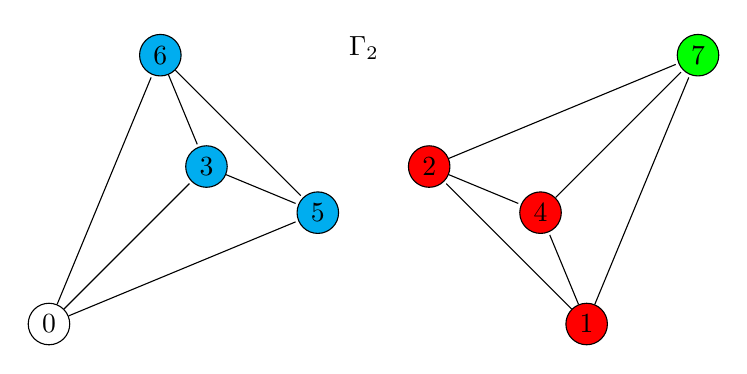
\begin{tikzpicture}[shorten >=1pt,auto,node distance=2cm,
				thin,main node/.style = {circle,draw, inner sep = 0pt, minimum size = 15pt}]
				
				\node[main node,fill=white] (1) {0};
				\node [right of = 1](2) {};
				\node [above of = 1](3) {};
				\node[main node,fill=cyan] [right of = 3](4) {3};
				\node [above right of = 1](5) {};
				\node[main node,fill=cyan] [right of = 5](6) {5};
				\node[main node,fill=cyan] [above of = 5] (7) {6};
				\node [right of = 7](8) {};
				
				\node [below right of =6] (11) {};
				\node[main node,fill=red] [right of = 11](12) {1};
				\node[main node,fill=red] [above of = 11](13) {2};
				\node [right of = 13](14) {};
				\node[main node,fill=red] [above right of = 11](15) {4};
				\node [right of = 15](16) {};
				\node [above of = 15] (17) {};
				\node[main node,fill=green] [right of = 17](18) {7};
				\node at (4,3.5) (9) {$\Gamma_2$};
				
				\path[-]
				(1)edge node {} (4)
				edge node {} (6)
				edge node {} (7)
				(12)edge node {} (13)
				edge node {} (15)
				edge node {} (18)
				(13)edge node {} (15)
				edge node {} (18)
				(4) edge node {} (6)
				(7) edge node {} (4)
				edge node {} (6)
				(15) edge node {} (18);
				\end{tikzpicture}
				\end{aligned}$}\end{center}
			For each of the two components we find a subscheme isomorphic to $K_4$.
		\begin{center}\scalebox{.7}{$\begin{aligned}
				\begin{tikzpicture}[shorten >=1pt,auto,node distance=2cm,
				thin,main node/.style = {circle,draw, inner sep = 0pt, minimum size = 15pt}]
				
				\node[main node,fill=white] (1) {0};
				\node[main node,fill=cyan] [right of = 3](4) {1};
				\node[main node,fill=cyan] [right of = 5](6) {2};
				\node[main node,fill=cyan] [above of = 5] (7) {3};
				\node at (2,4.5) (9) {$\Gamma_0^\prime$};
				
				\path (1) edge [in=120,out=145,loop] ();
				\path (4) edge [in=120,out=145,loop] ();
				\path (6) edge [in=120,out=145,loop] ();
				\path (7) edge [in=120,out=145,loop] ();
				
				\end{tikzpicture}\qquad\qquad
				\begin{tikzpicture}[shorten >=1pt,auto,node distance=2cm,
				thin,main node/.style = {circle,draw, inner sep = 0pt, minimum size = 15pt}]
				
				\node[main node,fill=white] (1) {0};
				\node[main node,fill=cyan] [right of = 3](4) {1};
				\node[main node,fill=cyan] [right of = 5](6) {2};
				\node[main node,fill=cyan] [above of = 5] (7) {3};
				\node at (2,4.5) (9) {$\Gamma_1^\prime$};
				
				\path[-]
				(1)edge node {} (4)
				edge node {} (6)
				edge node {} (7)
				(4) edge node {} (6)
				(7) edge node {} (4)
				edge node {} (6);
				\end{tikzpicture}
				\end{aligned}$}\end{center}
			The quotient scheme is found by collapsing each component to a single point, giving an association scheme isomorphic to $K_2$.
			\begin{center}\scalebox{.7}{$\begin{aligned}
			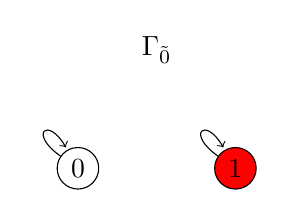
\begin{tikzpicture}[shorten >=1pt,auto,node distance=2cm,
			thin,main node/.style = {circle,draw, inner sep = 0pt, minimum size = 15pt}]
			
			\node[main node,fill=white] (1) {0};
			\node[main node,fill=red] [right of = 1](2) {1};
			\node at (1,1.5) (9) {$\Gamma_{\tilde{0}}$};
			
			\path (1) edge [in=120,out=145,loop] ();
			\path (2) edge [in=120,out=145,loop] ();
			
			\end{tikzpicture}\qquad\qquad
			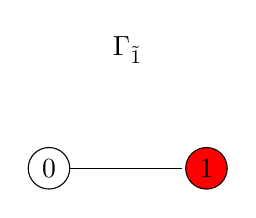
\begin{tikzpicture}[shorten >=1pt,auto,node distance=2cm,
			thin,main node/.style = {circle,draw, inner sep = 0pt, minimum size = 15pt}]
			
			\node[main node,fill=white] (1) {0};
			\node[main node,fill=red] [right of = 1](2) {1};
			\node at (1,1.5) (9) {$\Gamma_{\tilde{1}}$};
			
			\path[-]
			(1)edge node {} (2);
			\end{tikzpicture}
		\end{aligned}$}\end{center}
	Similarly, the system of imprimitivity given by $\cI_2 = \left\{0,3\right\}$ results in the following components of $\Gamma_3$:
	\begin{center}\scalebox{.7}{$\begin{aligned}
			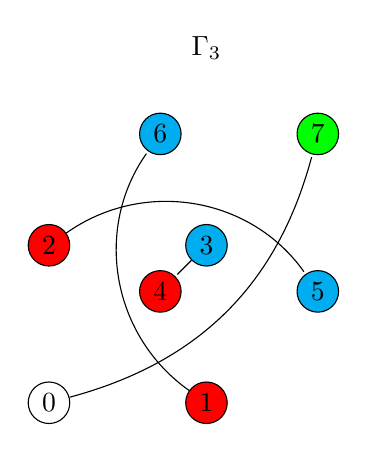
\begin{tikzpicture}[shorten >=1pt,auto,node distance=2cm,
			thin,main node/.style = {circle,draw, inner sep = 0pt, minimum size = 15pt}]
			
			\node[main node,fill=white] (1) {0};
			\node[main node,fill=red] [right of = 1](2) {1};
			\node[main node,fill=red] [above of = 1](3) {2};
			\node[main node,fill=cyan] [right of = 3](4) {3};
			\node[main node,fill=red] [above right of = 1](5) {4};
			\node[main node,fill=cyan] [right of = 5](6) {5};
			\node[main node,fill=cyan] [above of = 5] (7) {6};
			\node[main node,fill=green] [right of = 7](8) {7};
			\node at (2,4.5) (9) {$\Gamma_3$};
			
			\path[-]
			(1) edge [bend right] node {} (8)
			(2) edge [bend left=45] node {} (7)
			(3) edge [bend left=45] node {} (6)
			(4) edge node {} (5);
			\end{tikzpicture}
			\end{aligned}$}\end{center}
		Each component here results in a subscheme isomorphic to $K_2$.
		\begin{center}\scalebox{.7}{$\begin{aligned}
				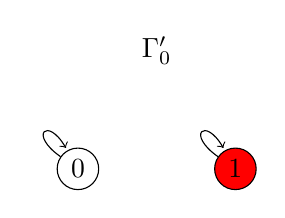
\begin{tikzpicture}[shorten >=1pt,auto,node distance=2cm,
				thin,main node/.style = {circle,draw, inner sep = 0pt, minimum size = 15pt}]
				
				\node[main node,fill=white] (1) {0};
				\node[main node,fill=red] [right of = 1](2) {1};
				\node at (1,1.5) (9) {$\Gamma_0^\prime$};
				
				\path (1) edge [in=120,out=145,loop] ();
				\path (2) edge [in=120,out=145,loop] ();
				
				\end{tikzpicture}\qquad\qquad
				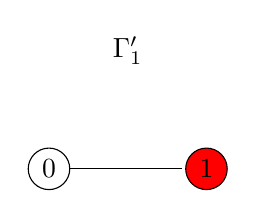
\begin{tikzpicture}[shorten >=1pt,auto,node distance=2cm,
				thin,main node/.style = {circle,draw, inner sep = 0pt, minimum size = 15pt}]
				
				\node[main node,fill=white] (1) {0};
				\node[main node,fill=red] [right of = 1](2) {1};
				\node at (1,1.5) (9) {$\Gamma_1^\prime$};
				
				\path[-]
				(1)edge node {} (2);
				\end{tikzpicture}
				\end{aligned}$}\end{center}
			Finally, the quotient scheme is isomorphic to $K_4$.
			
			\begin{center}\scalebox{.7}{$\begin{aligned}
					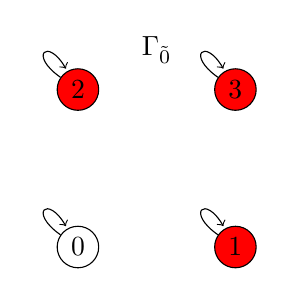
\begin{tikzpicture}[shorten >=1pt,auto,node distance=2cm,
					thin,main node/.style = {circle,draw, inner sep = 0pt, minimum size = 15pt}]
					
					\node[main node,fill=white] (1) {0};
					\node[main node,fill=red] [right of = 1](2) {1};
					\node[main node,fill=red] [above of = 1](3) {2};
					\node[main node,fill=red] [above of =2](4) {3};
					\node at (1,2.5) (9) {$\Gamma_{\tilde{0}}$};
					
					\path (1) edge [in=120,out=145,loop] ();
					\path (2) edge [in=120,out=145,loop] ();
					\path (3) edge [in=120,out=145,loop] ();
					\path (4) edge [in=120,out=145,loop] ();
					
					\end{tikzpicture}\qquad&\qquad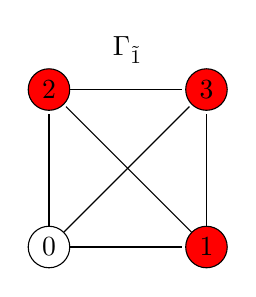
\begin{tikzpicture}[shorten >=1pt,auto,node distance=2cm,
					thin,main node/.style = {circle,draw, inner sep = 0pt, minimum size = 15pt}]
					
					\node[main node,fill=white] (1) {0};
					\node[main node,fill=red] [right of = 1](2) {1};
					\node[main node,fill=red] [above of = 1](3) {2};
					\node[main node,fill=red] [above of =2](4) {3};
					\node at (1,2.5) (9) {$\Gamma_{\tilde{1}}$};
					
					\path[-]
					(1) edge node {} (2)
					edge node {} (3)
					edge node {} (4)
					(2) edge node {} (3)
					edge node {} (4)
					(3) edge node {} (4);
					\end{tikzpicture}
					\end{aligned}$}\end{center}
	\section{Polynomial schemes}\label{poly}
	In this section we define and develop the notion of polynomial association schemes. We again present two dual concepts, $P$-polynomial and $Q$-polynomial though we will focus primarily on the $Q$-polynomial case outside of this section. Let $(X,\cR)$ be a $d$-class association scheme. We say $(X,\cR)$ is \emph{$Q$-polynomial}, or \emph{cometric}, if there exists an ordering of the Schur idempotents, say $E_0,E_1,\dots,E_d$, such that the Krein parameters satisfy the following conditions:
	\begin{enumerate}
		\item $q^k_{ij} = 0$ whenever $k>i+j$, and
		\item $q^k_{ij} > 0$ whenever $k = i+j$.
	\end{enumerate}
	We note that while this requirement, with Lemma \ref{kitchensink} $(iii'),(iv')$, requires more constraints than are listed here, it is sufficient to check only the above for $0\leq i,j,k\leq d$. In fact, it is sufficient to check only the above conditions with $i=1$ (see \cite[Prop.\ 2.7.1]{Brouwer1989}). Thus we may characterize $Q$-polynomial association schemes as exactly those for which there exists an eigenspace ordering for which the Krein array ($L_1^*$) is irreducible tridiagonal. When this occurs, we find that $\BMA = \left<E_1\right>$; that is, $E_1$ generates our entire Bose-Mesner algebra using Schur products. Then we may define single variable polynomials $q_k(t)$ of degree $k$ so that $Q_{ik} = q_k\left(Q_{i1}\right)$ for $0\leq i,k\leq d$ or equivalently $E_k = \frac{1}{\vert X\vert}q_k\circ\left(\vert X\vert E_1\right)$ (again see \cite[Prop.\ 2.7.1]{Brouwer1989}). This immediately implies that $E_1$ has $d+1$ distinct entries and we find it convenient to order the relations according to these values so that $Q_{01}>Q_{11}>\dots>Q_{d1}$; we call this the \emph{natural ordering} with respect to the $Q$-polynomial ordering $E_0,E_1,\dots,E_d$. As is suggested by this definition, it is possible to find multiple $Q$-polynomial orderings for the same association scheme. Suzuki showed (\cite{Suzuki1998-2}) however that, with the exception of cycles, any $Q$-polynomial association scheme has at most two $Q$-polynomial orderings. We say a $Q$-polynomial association scheme is \emph{$Q$-bipartite} if the Krein parameters fulfill the additional requirement $q^k_{ij} = 0$ whenever $i+j+k\notin 2\bbZ$. We find in this case that $\left\{E_i\right\}_{i\in 2\bbZ}$ serves as a Schur-closed subalgebra. Additionally we say a $Q$-polynomial scheme is \emph{$Q$-antipodal} if $q^k_{dd} = 0$ whenever $k\notin\left\{0,d\right\}$ and thus $\left\{E_0,E_d\right\}$ is a Schur-closed subalgebra. Each case results in a system of imprimitivity; the following theorem states that these are the only possible systems of imprimitivity for $Q$-polynomial association schemes.
	\begin{thm}[\cite{Suzuki1998},\cite{Cerzo2009},\cite{Tanaka2011}] \label{suzukiimprim} Suppose $(X,\mathcal{R})$ is an imprimitive cometric association scheme with $Q$-polynomial ordering $E_0,\dots,E_d$ and natural ordering $A_0,\dots,A_d$. Then one of the following holds:
	\begin{enumerate}[label=(\roman*)]
		\item $(X,\mathcal{R})$ is $Q$-bipartite and $\mathcal{J} = \left\{0,2,4,\dots\right\}$, $\mathcal{I} = \left\{0,d\right\}$;
		\item $(X,\mathcal{R})$ is $Q$-antipodal and $\mathcal{J} = \left\{0,d\right\}$, $\mathcal{I} = \left\{0,2,4,\dots\right\}$.
	\end{enumerate}
	\end{thm}
	The original theorem in \cite{Suzuki1998} allowed for two exceptional cases, one with $d=4$ and another with $d=6$. These two cases were later ruled out in \cite{Cerzo2009} and \cite{Tanaka2011} respectively.
	
	We now consider the dual definition, $P$-polynomial association schemes. Again let $(X,\cR)$ be a $d$-class association scheme. We say $(X,\cR)$ is \emph{$P$-polynomial}, or \emph{metric}, if there exists an ordering of the relations, say $A_0,A_1,\dots,A_d$, such that the intersection numbers satisfy the following conditions:
	\begin{enumerate}
		\item $p^k_{ij} = 0$ whenever $k>i+j$, and
		\item $p^k_{ij} > 0$ whenever $k = i+j$.
	\end{enumerate}
	As before we find that it is sufficient to check the above conditions only when $i=1$ (\cite[Prop.\ 2.7.1]{Brouwer1989}) and thus an association scheme is $P$-polynomial if and only if there exists an ordering of the relations for which the intersection array $(L_1)$ is irreducible tridiagonal. In this case we find that $\BMA= \left<A_1\right>$ and it is therefore common to consider a $P$-polynomial scheme synonymous with $\Gamma_1$--a \emph{distance regular graph}, noting that $(x,y)\in R_i$ if and only if $d_\Gamma(x,y) = i$. We find analogous results as we saw in the $Q$-polynomial case with \cite[Theorem 4.2.12]{Brouwer1989},\cite{Taylor1978} giving that any $P$-polynomial association scheme has at most two $P$-polynomial orderings. Further we may define \emph{$P$-bipartite} (or more commonly \emph{bipartite}) and \emph{$P$-antipodal} (\emph{antipodal}) as those schemes for which $p^k_{ij}\neq 0$ implies $i+j+k\in 2\bbZ$ and $p^k_{dd}\neq 0$ implies $k\in\left\{0,d\right\}$ respectively. For these schemes we again find systems of imprimitivity however this time $\mathcal{I} = \left\{0,2,4,\dots\right\}$ and $\mathcal{J} = \left\{0,d\right\}$ correspond to the bipartite scheme while $\mathcal{I} = \left\{0,d\right\}$ and $\mathcal{J} = \left\{0,2,4,\dots\right\}$ for the antipodal scheme. As before we find that these systems of imprimitivity are all that can occur for $P$-polynomial schemes (\cite{Smith1971},\cite{Gardiner1980}).
	
	Despite the close connection between $P$-polynomial and $Q$-polynomial association schemes, we note that many of the theorems mentioned here in the $P$-polynomial case predate their $Q$-polynomial analogues by as much as 30 years. Further there are many other theorems which are known to be true for metric schemes whose $Q$ analogues have yet to be proven. For instance Taylor and Levingston showed in 1978 (\cite{Taylor1978}) that the sequence $k_0,k_1,\dots,k_d$ is unimodal, however the $Q$-analogue: the sequence $m_0,m_1,\dots,m_d$ is unimodal, remains a conjecture to this day. Chapter 6 of \cite{Brouwer1989} details the known examples of distance regular graphs at that time--all tables mentioned here appear in that chapter. Here they list 21 classical parameter sets (Tables 6.1 \& 6.2), 15 of which correspond to infinite families, three folded classical graphs (Table 6.3), nine near regular polygons including the generalized polygons (Tables 6.5 \& 6.6), as well as 20 more primitive distance regular graphs (Tables 6.8 \& 6.9). Further they give the known bipartite and antipodal examples (Tables 6.9 \& 6.10 resp.). On the $Q$-polynomial side however, \cite{Martin2007} lists the $Q$-polynomial association schemes known in 2007: those that are also $P$-polynomial as well as four infinite families and 22 sporadic examples. Concerning the association schemes which are both metric and cometric, we note the following conjecture of Bannai and Ito.
	\begin{conj*}[Bannai \& Ito] 
		For $d$ sufficiently large, a primitive association scheme with $d$ classes is metric if and only if it is cometric.
	\end{conj*}
	With this conjecture in mind, we expect that as $d$ grows, the fraction of $Q$-polynomial schemes which are not also $P$-polynomial should diminish. However as can be seen by the tables hosted by Williford \cite{Williford} there is still much work to be done for small $d$. Note every $2$-class association scheme (strongly regular graphs) is automatically both metric and cometric, thus we will primarily focus on schemes which are have at least three classes.
	
	\section{Further background for cometric schemes}\label{qpolythms}
	Here we list a few extra results for cometric schemes which will be useful for the later chapters. It is likely that this section will get scrapped and the results will be moved to their respective chapters where they are useful.
	\begin{thm}\cite[Theorem.~1.3.1.(iii)]{Brouwer1989} Whenever $\mu>0$, the parameters of a strongly regular graph may be expressed in terms of $r$, $s$, and $\mu$ as
		\[k = \mu-rs, \qquad v = \frac{(k-r)(k-s)}{\mu},\qquad \lambda = \mu+r+s.\]
	\end{thm}
	\begin{thm}\cite{Delsarte1973} 
		Let $\Gamma$ be a strongly regular graph with $v$ vertices, valency $k$, and smallest eigenvalue $-m$. If $C$ is a coclique of $\Gamma$, then
		\[\vert C\vert\leq v\left(1+\frac{k}{m}\right))^{-1}, \]
		with equality if and only if every vertex $\gamma\notin C$ has the same number of neighbors (namely $m$) in $C$.
	\end{thm}
	\begin{thm}[\cite{Martin2007}] \label{mmw}The following are equivalent:
		\begin{enumerate}[label=(\roman*)]
			\item $(X,\mathbb{R})$ is imprimitive;
			\item for some $j>0$, $E_j$ has repeated columns;
			\item for some subset $\mathcal{I} = \left\{i_0=0,i_1,\dots,i_s\right\}$ of $\left\{0,1,\dots,d\right\}$ and some ordering of the vertices $\sum_{h=0}^s A_{i_h} = I_w\otimes J_r$ for integers $w$ and $r$ with $\vert X\vert=wr$, $1<w,r<\vert X\vert$;
			\item for some subset $\mathcal{J} = \left\{j_0=0,j_1,\dots,j_s\right\}$ of $\left\{0,1,\dots,d\right\}$ and some ordering of the vertices $\sum_{h=0}^s E_{j_h} = \frac{1}{r}\left(I_w\otimes J_r\right)$ for integers $w$ and $r$ with $\vert X\vert=wr$, $1<w,r<\vert X\vert$.
		\end{enumerate}
	\end{thm}
	Whenever $(iii)$ occurs, say with subset $\mathcal{I}$ as given in the theorem, we may partition our vertices into equivalence classes so that $x\sim y$ whenever $(x,y)\in R_i$ for some $i\in \mathcal{I}$. Let $X_1,\dots,X_w$ be the corresponding equivalence classes and define $\mathcal{R}' = \left\{R_i\in \mathcal{R} : i\in \mathcal{I}\right\}$. Then there exists \emph{subschemes} $(X_i,\mathcal{R}')$ for each equivalence class $X_i$. Further, we may define a \emph{quotient scheme} $(\tilde{X},\tilde{\mathcal{R}})$ of our original scheme with respect to $\mathcal{I}$ whose point set is the set of equivalence classes and whose relations are $R_{\tilde{i}} = \cup_{i\in \tilde{i}} R_i$ where each $\tilde{i} = \left\{0\leq j\leq d : p^x_{i,j} \text{ for }x\in \mathcal{I}\right\}$. Note that $\vert \tilde{\mathcal{R}}\vert = \vert \mathcal{J}\vert$ where $\mathcal{J}$ is the subset from Theorem $3.1(iv)$.

	\begin{cor}
		\label{SRG}
		The quotient scheme of a 4-class $Q$-bipartite association scheme is a strongly regular graph.
	\end{cor}
	\begin{proof}
		From Theorem \ref{suzuki}, we know $\mathcal{J} = \left\{0,2,4\right\}$ and therefore the quotient scheme has two nontrivial relations, forcing it to be strongly regular.
	\end{proof}
	\begin{thm}[\cite{Brouwer2003},\cite{Martin2007}]
		\label{sym}
		If $(X,\mathcal{R})$ is $Q$-bipartite with $w$ dual bipartite classes of size $r$ each, then $r=2$. Under the natural ordering of relations, $\mathcal{I} = \left\{0,d\right\}$ and the sequence $m = Q_{01}>Q_{11}>\dots>Q_{d1}$ is symmetric about the origin. In particular, $Q_{\frac{d}{2},1} = 0$ whenever $d$ is even.
	\end{thm}
	\begin{cor}
		\label{evenpoly}
		If $(X,\mathcal{R})$ is $Q$-bipartite, then $Q_{i,j} = Q_{d-i,j}$ $(-Q_{d-i,j}$, resp.) whenever $j$ is even (odd).
	\end{cor}
	\begin{proof}
		$q_j(t)$ is even (odd) whenever $j$ is even (odd). Since $Q_{i,1} = -Q_{d-i,1}$ and $Q_{i,j} = q_j(Q_{i,1})$, the result follows.
	\end{proof}
Twins -- Make sure they are somewhere.